\documentclass[Proceedings]{ascelike}
\usepackage{graphicx}
\usepackage{amsmath}
\usepackage{amsfonts}
\usepackage{amssymb}
\usepackage{tikz}
\usetikzlibrary{shapes.geometric, arrows}
\tikzstyle{arrow} = [thick,->,>=stealth]
\tikzstyle{startstop} = [rectangle, rounded corners, minimum height =1cm, text centered, draw=black, fill=blue!10]
\usepackage[utf8]{inputenc}
\usepackage[T1]{fontenc}
\usepackage{authblk}
\usepackage[colorlinks=true,citecolor=red,linkcolor=black]{hyperref}
\usepackage[colorlinks=true,citecolor=red,linkcolor=black]{hyperref}


\begin{document}
%
% You will need to make the title all-caps
\title{A HYBRID CAR-FOLLOWING MODEL THAT EXPLAINS TRAFFIC BREAKDOWN AT A BOTTLENECK}
\author[1]{Paul J. Ossenbruggen} 
\author[2]{Eric M. Laflamme}
\affil[1]{Department of Civil Engineering, University of New Hampshire, Durham NH 03824. Email: pjo@unh.edu}
\affil[2]{ Department of Mathematics and Statistics, Plymouth State University, Plymouth, NH 03264}
\maketitle
\begin{abstract} Traffic data are inherently noisy. As the name implies unwanted. Historically, traffic noise has been  treated as a nuisance variable and ignored. It is now possible to introduce the effects of noise into the decision-making process with the advent of high speed computing and advances in statistics. The principal goals of this paper is to predict and explain traffic breakdown at a bottleneck with the aid of a stochastic model. A Brownian motion model is at the core of the model development. It is introduced into a car-following model structure where driver group behavior is assumed to be root cause of breakdown. Results from a controlled experiment are used to sustain the assumption. This model and a deterministic traffic dynamics model are incorporated into a \emph{hybrid} model to investigate a bottleneck where a two-lane freeway merges into one lane. This framework allows us to analyze the driver group behavior as the drivers' approach, pass through with the option of passing other vehicles, and exit a bottleneck. Two merging protocols are investigated, the zipper and side-by-side merge. Average wait time for a side-by-side merge is estimated to be more than 4.5 times greater  than  a zipper merge. Since drivers' are self optimizers, implementing a zipper merge traffic control regulation as a matter of policy is deemed infeasible. The feasibility of adapting the hybrid car-following model into an $ITS$ control system and for traffic safety studies are discussed.
\end{abstract}
\KeyWords{Traffic breakdown, car-following, congestion, control, intelligent systems,  stochastic processes }
%
     
\section{Introduction}
Predicting and explaining traffic breakdown at a bottleneck is main goal and focus of this paper. There is no argument that traffic mix, geometric design, traffic management and control, weather conditions are contributing factors in explaining a breakdown event. In this paper, they are assumed to play a secondary role. Driver group behavior,  an informal group of drivers with various driving skills, levels of alertness and aggressiveness and attitudes toward safety and risk, is assumed to play a central role. 

Another goal of this paper is describe the breakdown process as simply as possible. That means using analysis tools, mathematical models, that are easy to understand. To help in this regard, the paper focuses on bottleneck breakdown using two merging protocols, \emph{zipper} and \emph{side-by-side} merges.

\emph{Why is it so difficult to explain and reliably predict traffic breakdown?} Traffic data are extremely noisy (volatile). Historically, researchers have treated noise as a nuisance variable. This is an eloquent  approach because their \emph{deterministic} models can explain fundamental relationship between speed, traffic density and flow. These methods give an incomplete explanation of traffic breakdown. The  research literature is rich with attempts to bring more clarity to solving this complex problem.  Factors explaining breakdown and its consequences include: speed volatility  \cite{WAGNER20121384}; vehicle clustering and density \cite{CASTILLO2001367}   \cite{GALTIER2012167} \cite{KISH2000271} \cite{MAHNKE20051} \cite{WEITS1992115}; driver behavior and headway distribution  \cite{OU2018105}; and capacity, delay, control and rerouting \cite{HU2018254} \cite{SMULDERS1990221} \cite{VODOPIVEC201722}. 

In this paper, a concerted effort is made to introduce traffic noise into the analysis by using \emph{stochastic models}. Our effort requires that the breakdown process be dissected, analyzed and then resembled. The resulting model, which we call a \emph{hybrid car-following model,} consists of both deterministic and stochastic model components. This framework allows us to analyze the driver group behavior as the drivers' approach, pass through, pass other vehicles, and exit a bottleneck.

The paper is organized as follows. The \textbf{METHODS} section consists of two sub-sections. The first sub-section deals with issues associated identifying the root cause  of traffic breakdown and the challenges associated modeling its behavior. Topics include:  \emph{Driver Group Behavior and Merging Protocols}, \emph{A Controlled Experiment}, and \emph{A Stochastic Model of Speed}. The second sub-section is entitled \textbf{A Hybrid Car-Following Model Parts and Assembly,} which contain topics on \emph{A Safe Car-Following Rule}, \emph{A Time Varying Acceleration Model}, \emph{Simulating Reality}, and \emph{Estimating Performance}. The \textbf{DISCUSSION AND RESULTS} section is devoted to answering a series of questions about  the integrity of the hybrid car-following model and to demonstrating how  it used to estimate bottleneck delay and capacity. Topics include: \emph{Performance Benchmarks} and \emph{Traffic Management Strategies}. The \textbf{SUMMARY} section lists the  important assumptions and findings.


\section{Methods}

\subsubsection{Driver Group Behavior and Merging Protocols.} 

The following scenario is investigated. Ten vehicles, five vehicles traveling on  parallel lanes, moving in the same direction are forced to merge into one lane. See Figure \ref{schematic}. Given a traffic density of 60 vehicles per mile per lane(vpm), traffic breakdown is expected.  The assigned density exceeds the lane capacity of 45 vpm \cite{HCM2000}. 


Two merging protocols are investigated: (1) the \emph{zipper merge} and (2) the \emph{side-by-side merge.} \citeN{vanderbilt} describes the  zipper merge as a ``late merge'' in a sociological sense resulting in road rage. \citeN{mndot} describes the zipper merge as a means of controlling traffic. In this paper, we adopt the second description and then evaluate its performance. 


\begin{figure}
\centering
%\framebox[3.00in]{\rule[0in]{0in}{1.00in}}
\includegraphics[width = 5.5in]{Rplot02.pdf}
\caption{Schematic diagram of a bottleneck.}
\label{schematic}
\end{figure}

A zipper merge in this paper is considered to be the gold standard of traffic operation at a bottleneck.  Traffic controlled  in this manner is analogous to  closing a jacket zipper, say. A jacket closes flawlessly because the rows of zipper teeth are the same size, move at the same speed, are evenly spaced and perfectly aligned to allow the two tapes to link together without jamming. From a traffic operations point of view, this is optimum. There is no jamming or delay. See the $t-x$ trajectory of Fig \ref{zipmodel}. Compare it to side-by-side merge of Fig \ref{sbsmodel} where drivers are delayed. The subscripts $A$ and $D$ denote  vehicle arrival and departure at locations $x_e$ and $x_0$, the bottleneck entry location and lane drop location, respectively. The ten vehicles traveling on lanes 1 and 2 are denoted by the red and blue lines. 

Drivers are assumed to be self optimizers.  They operate their vehicles to minimize their individual travel time, thus the group tends to be uncooperative and more prone to drive side-by-side. At the same time, individual drivers do it safely to avoid traffic accidents. For example, drivers traveling on upstream parallel lanes drive side-by-side feel secure and feel safe driving in this manner. Tailgaters, obviously, feel safe driving this way. Whether or not a driver is a tailgater, one of the drivers must yield to avoid crashing when reaching a bottleneck. A side-by-side merge is deemed to be a sub-optimum form of driving because traffic is interrupted and drivers must decelerate.  

\begin{figure}
\centering
%\framebox[3.00in]{\rule[0in]{0in}{1.00in}}
\includegraphics[width = 5.5in]{Rplot01.pdf}
\caption{A time-space trajectory of a ``zipper merge.''}
\label{zipmodel}
\end{figure}


\begin{figure}
\centering
%\framebox[3.00in]{\rule[0in]{0in}{1.00in}}
\includegraphics[width = 5.5in]{Rplot04.pdf}
\caption{A time-space trajectory of a ``side-by-side merge.''}
\label{sbsmodel}
\end{figure}


\begin{figure}
\centering
%\framebox[3.00in]{\rule[0in]{0in}{1.00in}}
\includegraphics[width = 5.5in]{Rplot09.pdf}
\caption{A sample time-space trajectory of a ``zipper merge'' produced by the hybrid car-following simulation model.}
\label{stochmodel}
\end{figure}

These two scenarios, zipper and side-by-side merge, described in these figures, use deterministic mathematical models derived from fundamental principles of traffic engineering. Neither model describes the situation observed in the field.  Vehicles traveling in a zipper merge configuration will not breakdown. No delay is predicted by this model.    The side-by-side model is described to be  an orderly process with some minor delay. While the second scenario may seem a bit more realistic than the first one, both models are considered unacceptable for explaining breakdown. Regardless, they prove useful and are not disregarded. They useful level of performance estimates that are used as benchmarks for comparison.


\subsubsection{A Controlled Experiment}

Since deterministic models cannot  adequately explain traffic breakdown observed in the field,  traffic breakdown event is analyzed as a stochastic process.   That means finding a  mathematical model that can adequately describe bottleneck breakdown. Experimental evidence shows  a breakdown is caused by  the drivers. Drivers, who are instructed to drive at a fixed speed $u$ and agree to do so, are unable to follow this simple instruction \cite{1367-2630-10-3-033001}. 

The experiment was conducted on a ring  road with circumference length $l$ and  a fixed number of  vehicles  $n$. The traffic density is $k = n/l$, a constant. At the start of the experiment, the vehicles were evenly spaced with three vehicle lengths of separation between them. After a few seconds, the drivers were unable to maintain the fixed speed $u$. Speeds became unstable, vehicles interacted and the traffic broke down.  The observed speed of an individual vehicle or group of vehicles can be averaged, which is denoted as $\bar{u}$, and its standard deviation estimated, which is denoted as $\sigma_U$ and call speed volatility.  

The \emph{root cause of traffic breakdown in this experiment} is twofold: (1) the drivers' inability to maintain  a fixed speed $u$ (2) and density $k$. Traffic density must be sufficiently large to cause vehicle interaction; otherwise, the vehicles will act independently and no breakdown will occur. The importance of this finding cannot be overemphasized. It shows a causal relationship between driver group behavior and breakdown.

\subsubsection{A Stochastic Model of Speed}

To explain this behavior with a speed model, speed is treated as a random variable $U$ where speed volatility, as before, is denoted as $\sigma_U$.  Since speed varies with time, the challenge is  to specify a stochastic speed model, The following model is investigated: $U(t) = f(\bar{u},\sigma_U,k,t)$ where $\bar{u}$ is the fixed speed that is specified for the ring road experiment, $\sigma_U$ is assumed to be a function of $k$. Since $n$ and $l$ are fixed, our first impulse is to treat $k$ as a constant. This assumption has great appeal for this paper because it meets our goal to explain breakdown with simple model structures. By treating  $k$ as a constant,  we derive the following flow model: $Q(t) = k \cdot U(t)$. Flow is an important measure of effectiveness and will be evidently used to estimate bottleneck capacity $c$.

Upon further investigation, we observe that vehicle interaction  takes place and vehicle clusters form and dissipate with time. Thus, $k$ cannot be a constant. The only time, density is a constant is when the experiment is initiated at time $t = 0$: $k_0 = n/l$. Unfortunately, the $Q(t) = k \cdot U(t)$ model must be rejected. For $t > 0$, density and flow must be treated as random variables. 

Both density and flow are modeled as $K(t)$ and $Q(t)$ diffusion models using field data averaged over fifteen time intervals, thus they are macroscale models  \cite{pjo2017}. The study shows traffic density is a more reliable predictor of traffic breakdown than flow, illustrating its  importance. Therefore,  a $K(t)$ diffusion model appears to be a good choice model for simulating traffic behavior on the ring road.  While it is possible  to calibrate a $K(t)$ diffusion model \cite{KISH2000271}, it is difficult to obtain field density data on a microscale scale. The same can be said for obtaining flow data of this scale. A different tactic is needed.

A \emph{Brownian bridge} model, $U(t) = f(\bar{u},\sigma_U,W,k,t)$ where $W$ = white noise, explains breakdown for the ring road experiment. As will be shown presently, this model  serves our needs (1) to explain breakdown at a bottleneck and (2) to estimate measures of performance at a bottleneck. The discussion above suggests stochastic process models of $K(t)$ and $Q(t)$ are needed. In lieu of deriving $K(t)$ and $Q(t)$ models, we use a car-following simulation model, a \emph{hybrid car-following model}, sampling and $t-x$ trajectories to obtain the information that we need. 

 
\subsection{A Hybrid Car-Following Model Parts and Assembly} 

This section is divided into two subsections: \emph{Parts} and \emph{Assembly}. The \emph{Parts} subsection focuses on mathematical model details and the \emph{Assembly} subsection focuses on how the parts work together. Examples are provided to help explain how the individual models work and how the assembled model integrates these individual models to produce practical output and insight. 

Traffic breakdown at a bottleneck is complicated and difficult to predict because of the effects of speed volatility. Figure \ref{stochmodel} shows its effects  at a bottleneck using a zipper merge protocol. The $t-x$ trajectories  shown here  is clearly different from the trajectories shown in Figure \ref{zipmodel}. Incidentally, the trajectories shown in Figure \ref{stochmodel} are derived from the hybrid car-following model. The trajectories shown in Figures \ref{stochmodel} and \ref{bbmodel}, a simulation involving two vehicles, a lead and following vehicle, are used throughout the paper to explain how the hybrid car-following model works.

\subsubsection{\underline{Parts} }

\begin{figure}
\centering
%\framebox[3.00in]{\rule[0in]{0in}{1.00in}}
\includegraphics[width = 5.5in]{Rplot03.pdf}
\caption{A sample draw from a Brownian bridge model of speed. }
\label{bbmodel}
\end{figure}


The  hybrid car-following model consists of the following parts: (1)  a \emph{Brownian bridge} model and (2) a \emph{time-varying acceleration} model. A Brownian bridge model  takes advantage of the properties defined by \emph{Brownian motion} model or  \emph{Wiener process} \cite{iacus}. Vehicle speed is estimated as:

\begin {equation}
u(t)  = \bar{u} + \sigma_U \cdot \big\{ W(t) - t/T \big\} \label{eq:eq1}
\end{equation}

\noindent where $t$, $\bar{u}$ and $\sigma_U$ are time, average speed and standard deviation of speed, respectively. \emph{Brownian motion} is denoted as $W(\Delta t) \sim \sqrt{\Delta t} \cdot N(0,1)$ and $N(0,1)$ denotes a standard normal probability distribution.  Given these data, vehicle locations are estimated using a time step approach:

\begin {equation}
x(t + \Delta t)  = x(t) + u(t) \cdot \Delta t  \label{eq:eq2}
\end{equation}

Data sets of speeds and locations for an \emph{individual} driver or vehicle $v$ are straightforwardly obtained by specifying $t = \{0,t_1,t_2,\ldots,T = t_{end}\}$, $u = \bar{u}$, $\sigma_U$ and $\Delta t$. Before proceeding, consider the two Brownian bridge speed traces of Figure \ref{bbmodel}.  The initial speed  and standard deviation  of $u$ = 53.1 mph and $\sigma_U$ = 5 mph are assigned to a lead and following vehicle. This simulation shows the lead vehicle start to accelerate at 10 seconds. The vehicle reaches a top speed at around 25 seconds and then it decelerates and returns to its initial speed of 53.1 mph.  A smooth curve drawn through the trace would more realistically depict how a driver would drive. 

The $t-x$ trajectory for this vehicle is relatively smooth despite the jagged  speed trace. The dashed line, a reference line, shows the vehicle trajectory  traveling at a constant speed of 53.1 mph. Another random draw from eq.(\ref{eq:eq1}) is made for a second vehicle, which we consider to be a following vehicle in this example. The $t-x$ trajectory of the following vehicle is similar to the lead vehicle. Of course, drawing a sample from the model could  be very different than the one described here even when $u$ and  $\sigma_U$  are assigned to same values.
 
Now take a look at the interaction between these two vehicles. The driver of the lead vehicle travels through the bottleneck merge zone without accelerating and then changes speed in the downstream zone. The driver of the following accelerates and passes the lead vehicle in the merge zone and then takes a lead position in the downstream zone. The following vehicle must pass the lead vehicle before it reaches $x$ = 0 to avoid a crash, which it does. The distance between the two vehicles are sufficient to avoid a crash. 

This simulation results in a vehicle passing event that is safe. Crossing trajectories in the downstream zone of one-lane are not permitted. If they cross, then crash is assumed to occur. All hybrid model simulations result in safe merges. If a simulation results in crossing trajectories or unsafe merges, then the following speed adjustments are made. Crossing trajectories are permitted in the upstream zone of two-lanes. However, that does not mean corrections are not needed.  Vehicles traveling in the same lane interact and are subject to safe driving rules. Traffic merging is complicated for model development because the wide variety and range interactions that can take place.

Words of warning. Side-by-side trajectories are often difficult to identify because their trajectories overlap. For the present, zipper trajectories are   used. Second, the \emph{Brownian bridge} model is sufficient to explain a ring road breakdown; the following two models are not needed.



\subsubsection{A Safe Car-Following Rule.} 

Independent draws are made using Eq.(\ref{eq:eq1}), thus the car-following trajectories shown in Figure \ref{bbmodel} were obtained strictly by chance. The trajectories are called \emph{desire-line trajectories.} No provision is made to classify drivers as aggressive, passive,  etc. However, the trajectories can be used to classify driver behavior if we wish. For practical application in transportation, it is  most important to have a wide variety of drivers represented in a simulation. In this example, the first or lead vehicle driver is considered  to be aggressive. The following vehicle driver  is considered to be a non-aggressive or passive driver  because he or she decelerates in the merge zone and tends to maintain a constant speed through most of the downstream zone.  

A safe car-following rule applied to these drivers and to all drivers in a simulation. The gap, the distance between lead vehicle and front bumper of the following vehicle, must be at least one-vehicle length for each ten mph. We denote it as $h_{safe}(u, l_{vehicle})$ where $u$ and $l_{vehicle}$ are speed and vehicle length. This rule applies everywhere except in the  merge zone. While the rule is simply enough to program, implementing it requires the rule to be applied differently in the upstream and downstream zones and to a variety of circumstances. 

\subsubsection{A Time Varying Acceleration Model.}

The smooth $t-x$ curve shown in Figure \ref{sbsmodel} is a good example on how a time varying acceleration model simulates driver behavior.  ``Realistically, acceleration is not a constant in time. Acceleration capabilities decrease as the speed increases. \cite{LiliBook}''  The model has the following form:

\begin {equation}
 \ddot{x} = \frac{d^2x}{dt^2} = \frac{du}{dt} =  a - b \cdot t \label{eq:eq3}
\end{equation}

\noindent where $a$ and $b$ are constants. 

This model is used in all hybrid model simulations. The $t-x$ simulation shown in Figure \ref{stochmodel} uses this relationship in several places. Since a $x$ trajectory derived with the function is a smooth curve and tends to blend in, it is difficult to discern.  The trajectory of vehicle (2,1) from between $t_1 \simeq$ 20 and $t_2 \simeq$ 28 seconds suggests the vehicle is closing in on vehicle (1,1) and must slowdown to avoid a crash over this time range. Stated another way, their desire-lines would cross or become too close together and violate the safe car-following rule. A correction is needed.

The obvious question is: How  are the constants $a$ and $b$ estimated? We need two equations to solve for the two unknowns. By integrating eq.(\ref{eq:eq3}), speed and location equations are obtained, which we denote as $u(a,b,t)$ and $x(a,b,t)$. Given the start and end times $t_1$ and $t_2$, we can estimate the start speed $u_1$, end speed $u_2$, start location $x_1$ and end location $u_2$ for the following vehicle at these times. These values are determined with the aid of the safe car-following rule:

\begin{eqnarray} 
u_{follow}(t_1) &=& u_{lead}(t_1) \\
u_{follow}(t_2) &=& u_{lead}(t_2) \\
x_{follow}(t_1) &=& x_{lead}(t_1) - h_{safe}(u_{lead}(t_1), l_{vehicle}) \\
x_{follow}(t_2) &=& x_{lead}(t_2) - h_{safe}(u_{lead}(t_2), l_{vehicle})  
\end{eqnarray}

\noindent By simplifying  the notation, $dt = t_2 - t_1$, $u_1 = u_{lead}(t_1)$,  $u_2 = u_{lead}(t_2)$, $x_1 = x_{lead}(t_1)$ and $x_2 = x_{lead}(t_2)$ and integrating the eq.(\ref{eq:eq3}), we write the speed and location functions for the following vehicle as:

\begin{eqnarray} 
u_2 &=& u_1 + a \cdot dt - \frac{b}{2} \cdot dt^2 \\
x_2 &=& x_1 + u_1 \cdot dt + \frac{a}{2}  \cdot dt^2 - \frac{b}{6} \cdot dt^3  
\end{eqnarray}

\noindent Factor the unknowns $a$ and $b$, rearrange the equations, and the  write them in matrix form:

\begin{equation}
  \begin{pmatrix}
 u_2 - u_1 \\
 x_2 - x_1 - u_1 \cdot dt
\end{pmatrix} =
\begin{pmatrix}
    dt & - \frac{dt^2}{2}\\
    \frac{dt^2}{2} & - \frac{dt^3}{6}
  \end{pmatrix} \cdot
  \begin{pmatrix}
    a \\
    b
    \end{pmatrix}
\end{equation}

\noindent Solve for $a$ and $b$ and then use eqs.(8) and (9) to forecast the values of $u_2$ and $x_2$ over the range from $t_1$ to $t_2$. 

\begin{figure}
\centering
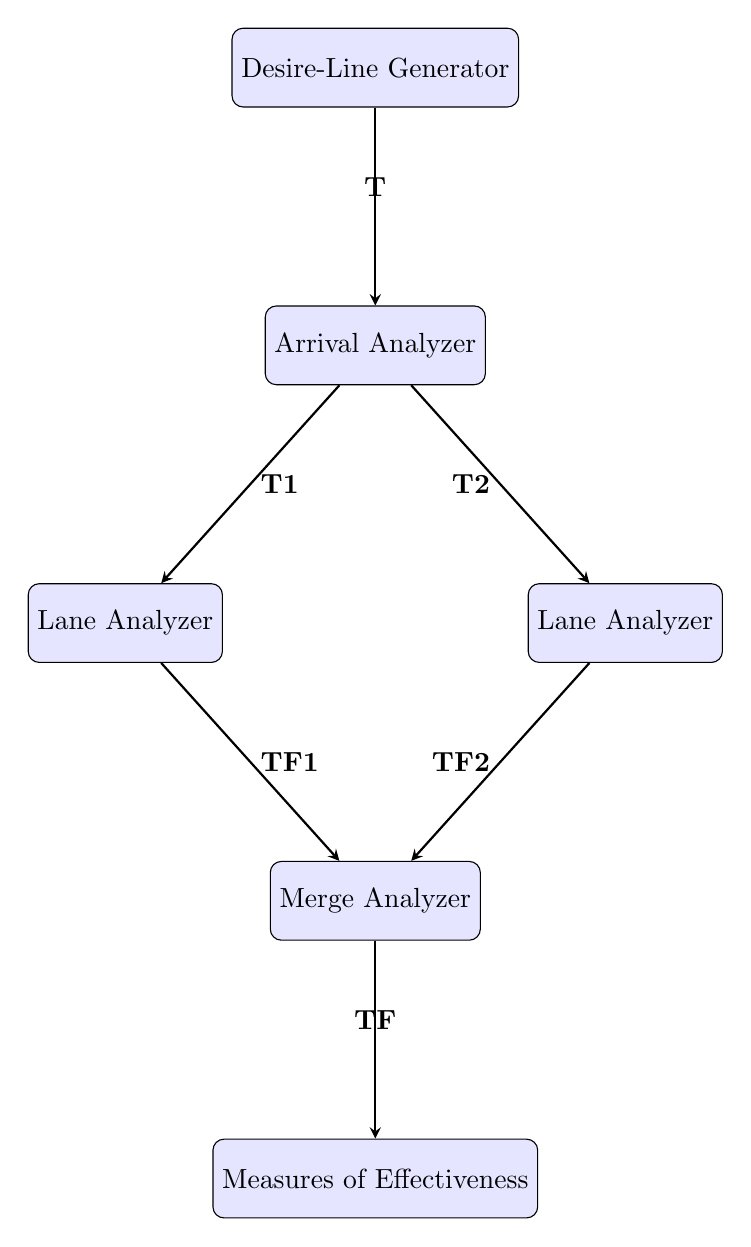
\begin{tikzpicture}[node distance=3cm] 
\node (start) [startstop] {Desire-Line Generator};
\node (bb) [startstop, below of = start, yshift =-15] {Arrival Analyzer};
\node (lane1) [startstop, below of = bb, yshift =-15, xshift = -1.25in] {Lane Analyzer};
\node (lane2) [startstop, below of = bb, yshift =-15, xshift = 1.25in] {Lane Analyzer};
\node (tuxfix) [startstop, below of = lane1, yshift =-15, xshift = 1.25in] {Merge Analyzer};
\node (mofe) [startstop, below of = tuxfix, yshift =-15, xshift = 0in] {Measures of Effectiveness};
\draw [arrow] (start) --  node[anchor=south] {$\mathbf{T}$} (bb);
\draw [arrow] (bb) --  node[anchor=west] {$\mathbf{T1}$} (lane1);
\draw [arrow] (bb) -- node[anchor=east] {$\mathbf{T2}$} (lane2);
\draw [arrow] (lane1) -- node[anchor=west] {$\mathbf{TF1}$} (tuxfix);
\draw [arrow] (lane2) -- node[anchor=east] {$\mathbf{TF2}$} (tuxfix);
\draw [arrow] (tuxfix) -- node[anchor=south] {$\mathbf{TF}$}  (mofe);
\end{tikzpicture}
\caption{Hybrid Car-Following Model flow chart.}
\label{flow}
\end{figure}


\subsubsection{\underline{Assembly}}


Previous examples demonstrate how these tools help explain breakdown for zipper and side-by-side merges at a bottleneck. These examples briefly mention desire-lines and gloss over their importance. Remember, if the desire-lines do not cross, then a crash does not take place. If they cross or are too close together, then a correction is made to secure \emph{safety.} Obviously, they are critically important.

How are these conditions detected? Start by inspecting the scatter plot of Figure \ref{bbmodelAD} and the cluster of points around the point $(\bar{k}_D, \bar{q}_D)$ and $k_{D_1},k_{D_2} \ldots,k_{D_9}$ and $q_{D_1},q_{D_2} \ldots,q_{D_9}$. All these values depend on the departure times when vehicles depart the merge zone and enter the downstream zone when vehicle spacing and speed are vitally important to \emph{safety.} Drivers do not know when they will reach $x_0$, thus these times are treated as random variables: $T_1, T_2,\ldots,T_{10}$. These times are not the arrival  times the drivers want (\emph{desire}).  They will plan their trip to arrive at times: $T^*_1, T^*_2,\ldots,T^*_{10}$. We call them \emph{desire} times. The  $T_{vehicle}$ and $T_{vehicle}^*$ times will, most likely, not match.  The  $T_{vehicle}$  times are modified   $T_{vehicle}^*$ times affected by uncertainty. Uncertainties associated with (1) drivers,  who drive in front of them on their travel lane, and with (2) drivers, who drive in front of them when they merge.

How does the hybrid car-following model find these times? The  \emph{desire}  times  $T_{vehicle}^*$ are determined by chance. Draws from the Brownian bridge model of eq.(\ref{eq:eq1}) and stored in a $\mathbf{T}$ matrix. It contains information about a vehicle's speed $u$ and location $x$ over time $t$. Using a time step of $\Delta t$ = 0.125 seconds for start time $t_{start} = 0$ to end time $t_{end} = 40$ seconds, $\mathbf{T}$  is a  321 $\times$ 21 matrix given $n$ = 10 vehicles with  $u(t)$ and $x(t)$ recordings for each vehicle.  The information in $\mathbf{T}$ may contain desire-lines that violate the safe car-following rule. They must be identified and corrected. The corrected information, which is found in a step-wise fashion,  is stored in matrices $\mathbf{T1}$, $\mathbf{T2}$, $\mathbf{TF1}$, $\mathbf{TF2}$ and $\mathbf{TF}$; matrices with the same dimension as $\mathbf{T}$. $\mathbf{1}$ and $\mathbf{2}$ refer to the lane numbers and $\mathbf{F}$ means \emph{fixed.}  In other words, corrected information is contained in the matrix.  The flow chart of Figure \ref{flow} outlines the procedure in finding the  $T_{vehicle}$ values and \emph{fixing} the $t-x$ trajectories that violate the safe car-following rule:

\begin{description}
\item [ Desire-Line Generator] produces a $\mathbf{T}$ matrix for $n$ =10 vehicles. $\mathbf{T}$ contains $n$ =10  $T_{vehicle}^*$ times but they are unknown values after performing this step.
\item [ Arrival Analyzer] sorts the information of $\mathbf{T}$ by lane number and stores it in $\mathbf{T1}$ and  $\mathbf{T2}$.
\item [ Lane Analyzer] independently inspects each following vehicle for safety violations from $\mathbf{T1}$ and  $\mathbf{T2}$. If a violation is found over some time range, the violation is corrected or fixed using the Time Varying Acceleration Model procedure given previously in the \textbf{Methods} section.  The information of $u(t)$ and $x(t)$  are replaced and stored in   the appropriate matrix $\mathbf{TF1}$ or  $\mathbf{TF2}$.
\item [ Merge Analyzer] merges the information in $\mathbf{TF1}$ or  $\mathbf{TF2}$. First, by ordering vehicle arrivals by arrival time at $x_0$ and stores them in $\mathbf{TF}$, contain values of  $T^*_1, T^*_2,\ldots,T^*_{10}$. Note that these values are  not the same values found in the Desire-Line Generator. Second, after performing similar steps to those given for the  Lane Analyzer step, corrections are made. This second set of corrections are stored in $\mathbf{TF}$. This matrix contains $T_1, T_2,\ldots,T_{10}$, the departure times from the bottleneck at $x_0$. These points are special because drivers realize by the time they reach location $x_0$ that corrections must be completed to proceed safely. In other words, drivers may take corrective action prior to reaching $x_0$ and before reaching $x_e$. 

\item [ Measure of Effectiveness] use the information contained in $\mathbf{TF}$ to estimate wait times $w$ and $t-x$ plots for a simulation.
\end{description}

\subsubsection{Simulating Reality.} 

Before discussing  measures of performance estimation, we feel it prudent to answer the following questions: 

\noindent \emph{What assurances can be offered to assure the hybrid car-following model simulates reality? }

 The ring-road experiment offers little doubt that vehicles that are closely spaced together cannot maintain a given speed and local queuing takes place and traffic breakdown occurs. The Brownian Bridge model successfully simulates this behavior. The model adds credence to the fact that speed volatility is strongly associated with driver group behavior. The Brownian Bridge model was  rigorously tested and found to satisfy fundamental principles of transportation engineering and match conditions observed in the field. The hybrid car-following model uses the Brownian Bridge model as its base, adds the notion that drivers are self optimizers, and other features, like a safe car-following rule and the time varying acceleration model, that simulate driver behavior. This model was tested. It passed the same tests as the Brownian Bridge model.

\noindent \emph{How is the model calibrated? } 

The Brownian Bridge and hybrid car-following model parameters of $u$ and $\sigma_U$ are not calibrated in the manner in which parameters of a probability model are. Maximum likelihood estimation (MLE) is a popular method. To use MLE, microscale field data are needed. Since this data is not available, it makes sense to use computer simulation. Thus, the parameters $u$, $\sigma_U$ and $\Delta t$ are assigned.  If the $\Delta t$ is assigned a value that is too long, then round-off error becomes an issue. Imagine for the moment that our data are not simulated but collected using aerial photography. Say, photographs are taken every  $\Delta t$ = 0.125 second,  vehicles identified, and $t-x$ trajectories plotted. Data derived from aerial photographs at this time-scale would be considered ideal and therefore, $\Delta t$ = 0.125 second is considered for computer simulation.

\noindent \emph{What are its limitations?} 

The hybrid car-following model is limited to zipper and side-by-side merges at a bottleneck where vehicles are  evenly spaced at time $t$ = 0. All drivers are assumed to drive safely as specified in the safe car-following rule. Therefore, the effect of tailgating, for example cannot be investigated. This feature as well as  weaving at a freeway interchange can be added. 

\subsubsection{Estimating Performance.} 


\begin{figure}
\centering
%\framebox[3.00in]{\rule[0in]{0in}{1.00in}}
\includegraphics[width = 5.5in]{Rplot05.pdf}
\caption{Results for the  ``zipper merge'' shown in Figure \ref{stochmodel}.}
\label{bbmodelAD}
\end{figure}

Capacity and delay are arguably the most important performance measures that define a transportation facility. They are estimated with the aid of the hybrid car-following model. We assume that the bottleneck is a queuing system, the same way a toll booth is a queuing system \cite{banks:1998}. The merge zone shown in Figure \ref{schematic} is defined to be the system server where vehicles arrive at $x_e$ and depart at $x_0$. The wait  time $w$ is the service time, the  travel time from points $x_e$ to $x_0$ or  $w = t_D - t_A$, the difference between the departure $D$ and arrival $A$ times. 

The task to estimate $w$  is made easier by using arrival  $A(t)$ and departure $D(t)$ rates.  The step plot shown in Figure \ref{bbmodelAD} are constructed with the information contained in $\mathbf{TF}$. The wait time for a given vehicle is $W_t = D(t) - A(t)$. The  time to travel through the bottleneck without delay is: $t^* = (x_0 - x_e)/u$.  Thus, $W'(t) = W(t) - t^*$ is an estimate of delay for a given vehicle. The averages of these respected estimates are reported as $w$ and $w'$ for a simulation.


The bottleneck capacity $c$ is the maximum flow through the bottleneck. Thus, $c = max(q_A,q_D)$, the maximum value of the arrival and departure flows.  Flows $q_A$ and  $q_D$ are estimated using the fundamental relationship $q = 1/h$ where $h$ is time headway between a lead and following vehicle and $h = t_{follower} - t_{leader}$. These times are contained in  $\mathbf{TF}$. Each follower/leader pair must be identified. For $n = 10$ vehicles, there are 9 pairs for $q_A$  and 9 pairs for $q_D$: $\{q_{D_1},q_{D_2},\ldots,q_{D_9}\}$ and $\{q_{A_1},q_{A_2},\ldots,q_{A_9}\}$.

The easiest way to identify these times is to use a $t-x$ trajectory plot. For $q_D$ at $x_0$, $h = t_2 - t_1$ for the first two vehicles is  identified by the $(t_1, x_1 = 0)$ and $(t_2, x_2 = 0)$ points for  $x_0 = 0$.    Repeat this procedure for each lead/follower pair and store the estimates. Flow $q_A$ at $x_e$ is estimated in the same way for $x_e$. The first estimate in the data set   $q_{A _1 } = 1/h $ for points $(t_1, x_1 = x_e)$, $(t_2, x_2 = x_e)$ and $h = t_2 - t_1$. Repeat and store the results. $q_D$ and $q_A$ are estimated as the averages of  $\{q_{D_1},q_{D_2},\ldots,q_{D_9}\}$ and $\{q_{A_1},q_{A_2},\ldots,q_{A_9}\}$, respectively.
 
Densities $k_D$ and $k_A$, which are of interest, are estimated using a similar averaging procedure using distance headways of $s$, the formula $k = 1/s$, and a modified identification procedure described above for distances. For example,  the first value in the data set $\{k_{D_1},k_{D_2},\ldots,k_{D_9}\}$   is estimated as $k_{D_1} = 1/s = x_2$ for points $(t_1, x_1 = 0)$ and $(t_1,  x_2)$. In contrast, the first value of the data set  $\{k_{A_1},k_{A_2},\ldots,k_{A_9}\}$ is estimated as $k_{A_1} = 1/s = 1/( x_2 - x_e)$ for points $(t_1,  x_e)$ and $(t_1,  x_2)$. The estimates $k_A$ and $k_D$ are averages of $\{k_{D_1},k_{D_2},\ldots,k_{D_9}\}$ and $\{k_{A_1},k_{A_2},\ldots,k_{A_9}\}$, respectively.

We will store these averages, $w, w', q_A, q_D, k_A, k_D$  in a performance vector $\mathbf{P}$. Capacity $c = max(q_A,q_D)$ is purposely is not listed in $\mathbf{P}$ because designating capacity for a single simulation, a single sample, makes no sense.  Just as real-world data are volatile and subject to uncertainty so are simulated data. To gain confidence in an estimate, more samples are drawn from the hybrid car-following model. The law of averages is used as a guide  \cite{freedman}. Two hundred  simulation runs, 100 runs for each merge type, are drawn. Summary statistics, means and standard errors (SE), are  listed in Table \ref{tab:tab2}. The Pairs Test will be discussed presently. 

The lower and upper bounds of the 95$\%$ C.I. (Confidence Interval) are listed. We can be about 95$\%$ confident that the true mean will lie somewhere within these bounds. For example, consider the 95$\%$ C.I.  of wait time $w$ for a side-by-side merge, (3.4,17.6). A driver can be about 95$\%$ confident that his or her wait time will be somewhere in this range. On average, the driver will expect a wait time of 10.5 seconds. Given the alleged benefits of a zipper merge, it is not surprising that the the average wait time is wait time is less than the side-by-side merge. In addition, its  95$\%$ C.I.  is tighter.

Now, we turn our attention to estimating a bottleneck capacity using the relationship $c = max(q_A,q_D)$. After inspecting the table, we declare the $c$ = 1903 vph is the best estimate of capacity. The side-by-side merge is more beneficial than the zipper merge. Given the Highway Capacity Manual guidelines, the estimate seems reasonable. However, our confidence in this estimate is shaky given its 95$\%$ C.I. is (841, 2965). The volatility in the simulation data affects the decision.


\section{Discussion and Results}

The \textbf{Methods} section is devoted to mathematical details. This section is devoted to practical matters. We will answer these important questions: ``What does an estimate reveal?'' ``Can an estimate be trusted?'' ``Is an estimate or a collection of estimates of any practical use?" 

We begin by looking at the simulation  of Figure \ref{stochmodel} once again and state: A \emph{typical breakdown} is impossible to define.  Why? One simulation does not tell the whole story of traffic breakdown. 

\noindent \emph{1. What can a single simulation tell us? }

Some vehicles pass others, some vehicles are constrained from passing, and some vehicles are unconstrained.   The first two vehicles, (1,1) and (2,1), experience no delay and have no affect on the following vehicles. If fact, both lead vehicles accelerate through the merge zone and separate themselves from the others. Even though  the speed  of the first two vehicles (1,1) and (2,1) exceed the initial speed of  $u$ = 53.1 mph, the average speed of all vehicles is $\bar{u}_D$ = 44.2 mph, which is well below 53.1 mph.  Consider the next two merging vehicles,  the blue and red line trajectories of  vehicles (1,2) and (2,2). Vehicle (2,2) reaches $x_0$ before vehicle (1,2), thus it goes first. Vehicle (1,2) catches up to vehicle (2,2) at around 18 seconds when it must limit its speed to that of the lead vehicle.  Since the safe car-following rule is applied, the driver of vehicle (1,2)  maintains a safe distance behind vehicle (2,2) in the downstream zone. These two vehicles affect the next four vehicles. Vehicles (2,5) and (2,4), on the other hand, seem to keep a safe distances in excess of that required by the safe car-following rule. Spillback takes place. The trajectories in the downstream zone are shown to fan outward.  

There is truth in the statement that a \emph{typical breakdown} is impossible to define. Six of the ten vehicles are found to be delayed by breakdown. The first two vehicles are accelerate and play no part in the breakdown. The last two vehicles may not part of the breakdown, but spillback may have some bearing their behavior. This breakdown is complicated by many factors. Next, the  average departure speed is $\bar{u}_D$ = 44.2 mph. The average of ten speed observations, which include a collection of free-flow and congested speeds. The speed estimate may overestimate the true congested speed. Thus, placing too much confidence in an estimate from a single sample or simulation can be misleading.  Sampling and the law of averages  presently above addresses this issue. At the same, inspecting a single simulation run helps explain the breakdown process.

\subsubsection{Performance Benchmarks.}

\noindent \emph{2. Given a zipper merge is considered the gold standard of transportation performance, should it promoted?}

 It offers a constant interrupted speed of $u_D$ = 53.1 mph,  traffic flow of $q_D$ = 3161 vph, and no delay, $w' = 0$ seconds. See Table \ref{tab:tab2}. Why? $\sigma_U$ = 0. The side-by-side merge offers a speed of $u_D$ = 39.2 mph, traffic flow of  $q_D$ = 2024 vph, and some delay, $w' = 0.7$ seconds per vehicle. Again, $\sigma_U$ = 0.  

 These figures offer conclusive evidence of the efficiency of a zipper merge. It has a capacity of $c = q_D$ = 3161 vph when the speed is fixed at $u_D$ = 53.1 mph. It is a much preferred alternate to a side-by-merge.  Based on these estimates, it seems like good policy to promote zipper merging.  The lofty promises given in Table \ref{tab:tab2} can be achieved only if  $\sigma_U$ = 0. At present, there is no technology that can achieve this end.    This statement does not mean that zipper merging should not be promoted. Furthermore, numbers matter in decision-making. For example, the capacity of the zipper merge  of $c$ = 3161 vph lies outside the 95$\%$ C.I. of (1151, 2457) given in Table \ref{tab:tab2}. The value of $c$ = 3161 vph can be considered an outlier.

\noindent \emph{3. Can stronger evidence be offered to support  zipper merging?}

A pairs test of significance can address this question. The null hypothesis states there is no difference in performance between the zipper and side-by-side merges. The alternative hypothesis suggests otherwise. Thus, any difference is due to chance. \citeN{freedman} warn: ``The \emph{P-value} of the test is the chance of getting a big test statistic - assuming the null hypothesis to be right. \emph{P} is not the chance the null hypothesis being right.'' With this mind, there is evidence to suggest that there is a difference in performance for $u_D, w$ and $w'$ favoring the zipper merge. The analysis suggests that it offers a faster average speed and lower wait times than a side-by-side merge. 

We previously declared that the bottleneck capacity is $c$ = 1903 vph. Since \emph{P-value} = 0.067, the pair test suggests that the evidence is not strong enough to claim a difference in the $q_D$ estimates. Thus, we stand by our previous decision, $c$ = 1903 vph. The result suggests that a zipper merge is less efficient than a side-by-side merge in maximizing traffic flow. Given the average wait time is estimated to be more than 4.5 times greater for a side-by-side merge than a zipper merge with questionable gains in capacity associated with side-by-side merging, the evidence supports zipper merging.

Moreover, doubling $\sigma_U$ to 10 mph results in gridlock. Hybrid car-following model simulations, like those shown of Figures \ref{sbsmodel}  and \ref{stochmodel}, show $t-x$ trajectories with zero slope indicating speeds are equal to zero. Incidentally, we chose the values of $u$ = 53.1 and  $\sigma_U$ = 5 mph to  simulate the bottleneck conditions in Salem, NH \cite{Laflamme2017}, \cite{Laflamme2018a}. Traffic delay as depicted in this paper are common. Gridlock was not.

 Since zipper merging benefits drivers, it makes sense to promote it. Given drivers are self optimizers, a promotional campaign is more than likely to fail. Naturally, this leads to the following question.
 
\subsubsection{Traffic Management Strategies.}

\noindent \emph{4. Can traffic noise be controlled?}

 Conceptually, it can be controlled  by applying \emph{Intelligent Transportation Systems} ($ITS$) in a smart city environment, an area that uses different types of electronic data collection sensors to supply information to manage resources: (1) Collect GPS floating car data \cite{KENDZIORRA2016198}, (2) Use a real-time, micro-scale forecast algorithm \cite{trieber}, and (3) Use GPS to transmit individualized ``optimized'' driver instruction. Floating car data are  real time, tracking data of $u_{vehicle}(t)$ and  $x_{vehicle}(t)$, which are transmitted using wireless technology and stored on a central controller computer \cite{tarnoff}. A real-time micro-scale forecast algorithm provides ``optimized'' $u_{driver}(t)$ and  $x_{driver}(t)$, provided by the tracking data. The ``optimized'' data are transmitted to on-board control installed in a vehicle \cite{5gaa}. The hybrid car-following model is a  micro-scale model that can be adapted to this purpose. 
 
 The hybrid car-following model can be adapted to suit the needs of $ITS$. It can also be used to study traffic weaving and tailgating where  safety is a critical concern. People interested in pursuing these efforts by using the hybrid car-following model are encouraged to do so. It is available online under the name \textbf{cartools}, a computer package written in \textbf{R}  \cite{cran}.   \textbf{cartools} is short for hybrid car-following model. The  code can be downloaded from GitHub  \cite{pjo2018}. A vignette is also available \cite{cartools}. 




\section{Summary}

Classical principles of transportation engineering and statistics are coupled with deterministic and stochastic models  to simulate traffic breakdown  using a car-following framework. The most important assumptions and findings are:


\begin{enumerate}
\item Traffic noise (speed volatility) is caused by individual drivers.
\item The root cause of traffic breakdown on a ring road and bottleneck is group driver behavior and high traffic density.
\item The hybrid car-following model simulations:
\begin{itemize}
\item Helps explain traffic behavior observed in the field.
\item Is a practical tool for evaluating traffic performance.
\end{itemize}
\item The hybrid car-following model, a micro-scale model,  can be adapted and used for real-time \emph{ITS} applications.
\end{enumerate}




\begin{table}
\caption{Stochastic Model Predictions}
\centering
\small
\begin{tabular}{|c|ccc|ccc|cc|}
 \hline
 \hline
&\multicolumn{3}{c|}{Side-by-Side Merge}&\multicolumn{3}{c|}{Zipper Merge}&\multicolumn{2}{c|}{Pairs Test}\\

 & Mean & SE & $95\%$ C.I. & Mean & SE & $95\%$ C.I. &  Mean Difference & $P-value$\\
\hline
$u_A$ at $x_e$ & 44.7& 12.9&(19.4,  69.9) & 52.3& 14.5& (23.9, 80.7) &-4.5 & 0.04\\
$k_A$ at $x_e$ & 70.2& 53.4& (-34.5,  175)& 63.3& 110 & (-152, 279)& 6.3 &0\\
$q_A$ at $x_e$ & 1134& 445& (262, 2006)& 1181& 265 & (662, 1700)& -47 & 0.64\\
\hline
$u_D$ at $x_0$ & 31.1& 6.0& (19.3, 42.86) & 44.3& 8.4&(27.8, 60.8)&-13.2 & 0\\
$k_D$ at $x_0$ & 43.7& 9.4& (25.3, 62.1)&37.4& 7.3 & (23.1, 51.7)&6.3 & 0\\
$q_D$ at $x_0$ & 1903& 542& (841, 2965)& 1804& 333 & (1151, 2457)&100 & 0.067\\
\hline
$w$     & 10.5 & 3.6 & (3.4, 17.6)& 7.9 & 2.3 & (3.39, 12.4)& 2.6 & 0 \\
$w'$     & 7.1 & 3.6 & (0.04, 14.2)& 1.5 & 2.3 & (-3.0, 6.0)& 2.6 & 0 \\
\hline
\hline
\end{tabular}
\label{tab:tab2}
\normalsize
\end{table}


\begin{table}
\caption{Deterministic Model Predictions}
\centering
\small
\begin{tabular}{|c|c|c|}
\hline
\hline
&Side-by-Side Merge&Zipper Merge\\
\hline
 $u_D$ at $x_0$  & 39.2 & 53.1 \\
 $k_D$ at $x_0$  & 41.7& 60.0 \\
 $q_D$ at $x_0$  & 2024&  3161 \\
 \hline
$w$     & 7.6 &   6.4 \\
$w'$     & 0.7 &  0  \\
 \hline
\hline
\end{tabular}
\label{tab:tab1}
\normalsize
\end{table}


\appendix\label{section:references}
%
\bibliography{CF}
%
\section{Notation}
\emph{The following symbols are used in this paper:}%\par\vspace{0.10in}
\nopagebreak
\par
\begin{tabular}{r  @{\hspace{1em}=\hspace{1em}}  l}
$v$                     & vehicle or driver number;\\
$n$                     & vehicle count;\\
$l$                      & length (feet);\\
$q$                    & flow (vph); \\
$k$                    & density, (vpm); \\
$u$                    & speed, (mph); \\
$x$                    & location (feet);      and\\
$t$                     & time (seconds).
\end{tabular}
%
\end{document}
